\documentclass{book}
\usepackage[utf8]{inputenc}
\usepackage{graphicx}
\usepackage{listings}
\usepackage{hyperref}
\usepackage{amsmath}
\newtheorem{definition}{Definition}


\begin{document}
\setlength{\parindent}{0cm}
\chapter{Git and GitHub}

intro

Explain what git and GitHub are and their purposes

\section{Config}

Cette section devrait déjà être faite, vous devriez déjà avoir un compte github, avoir téléchargé git et avoir configuré votre email. Si jamais ce n'est pas fait, voici comment le faire. 

Commencez par ouvrir votre terminal et taper "git" 

\begin{figure}[!h]
    \centering
    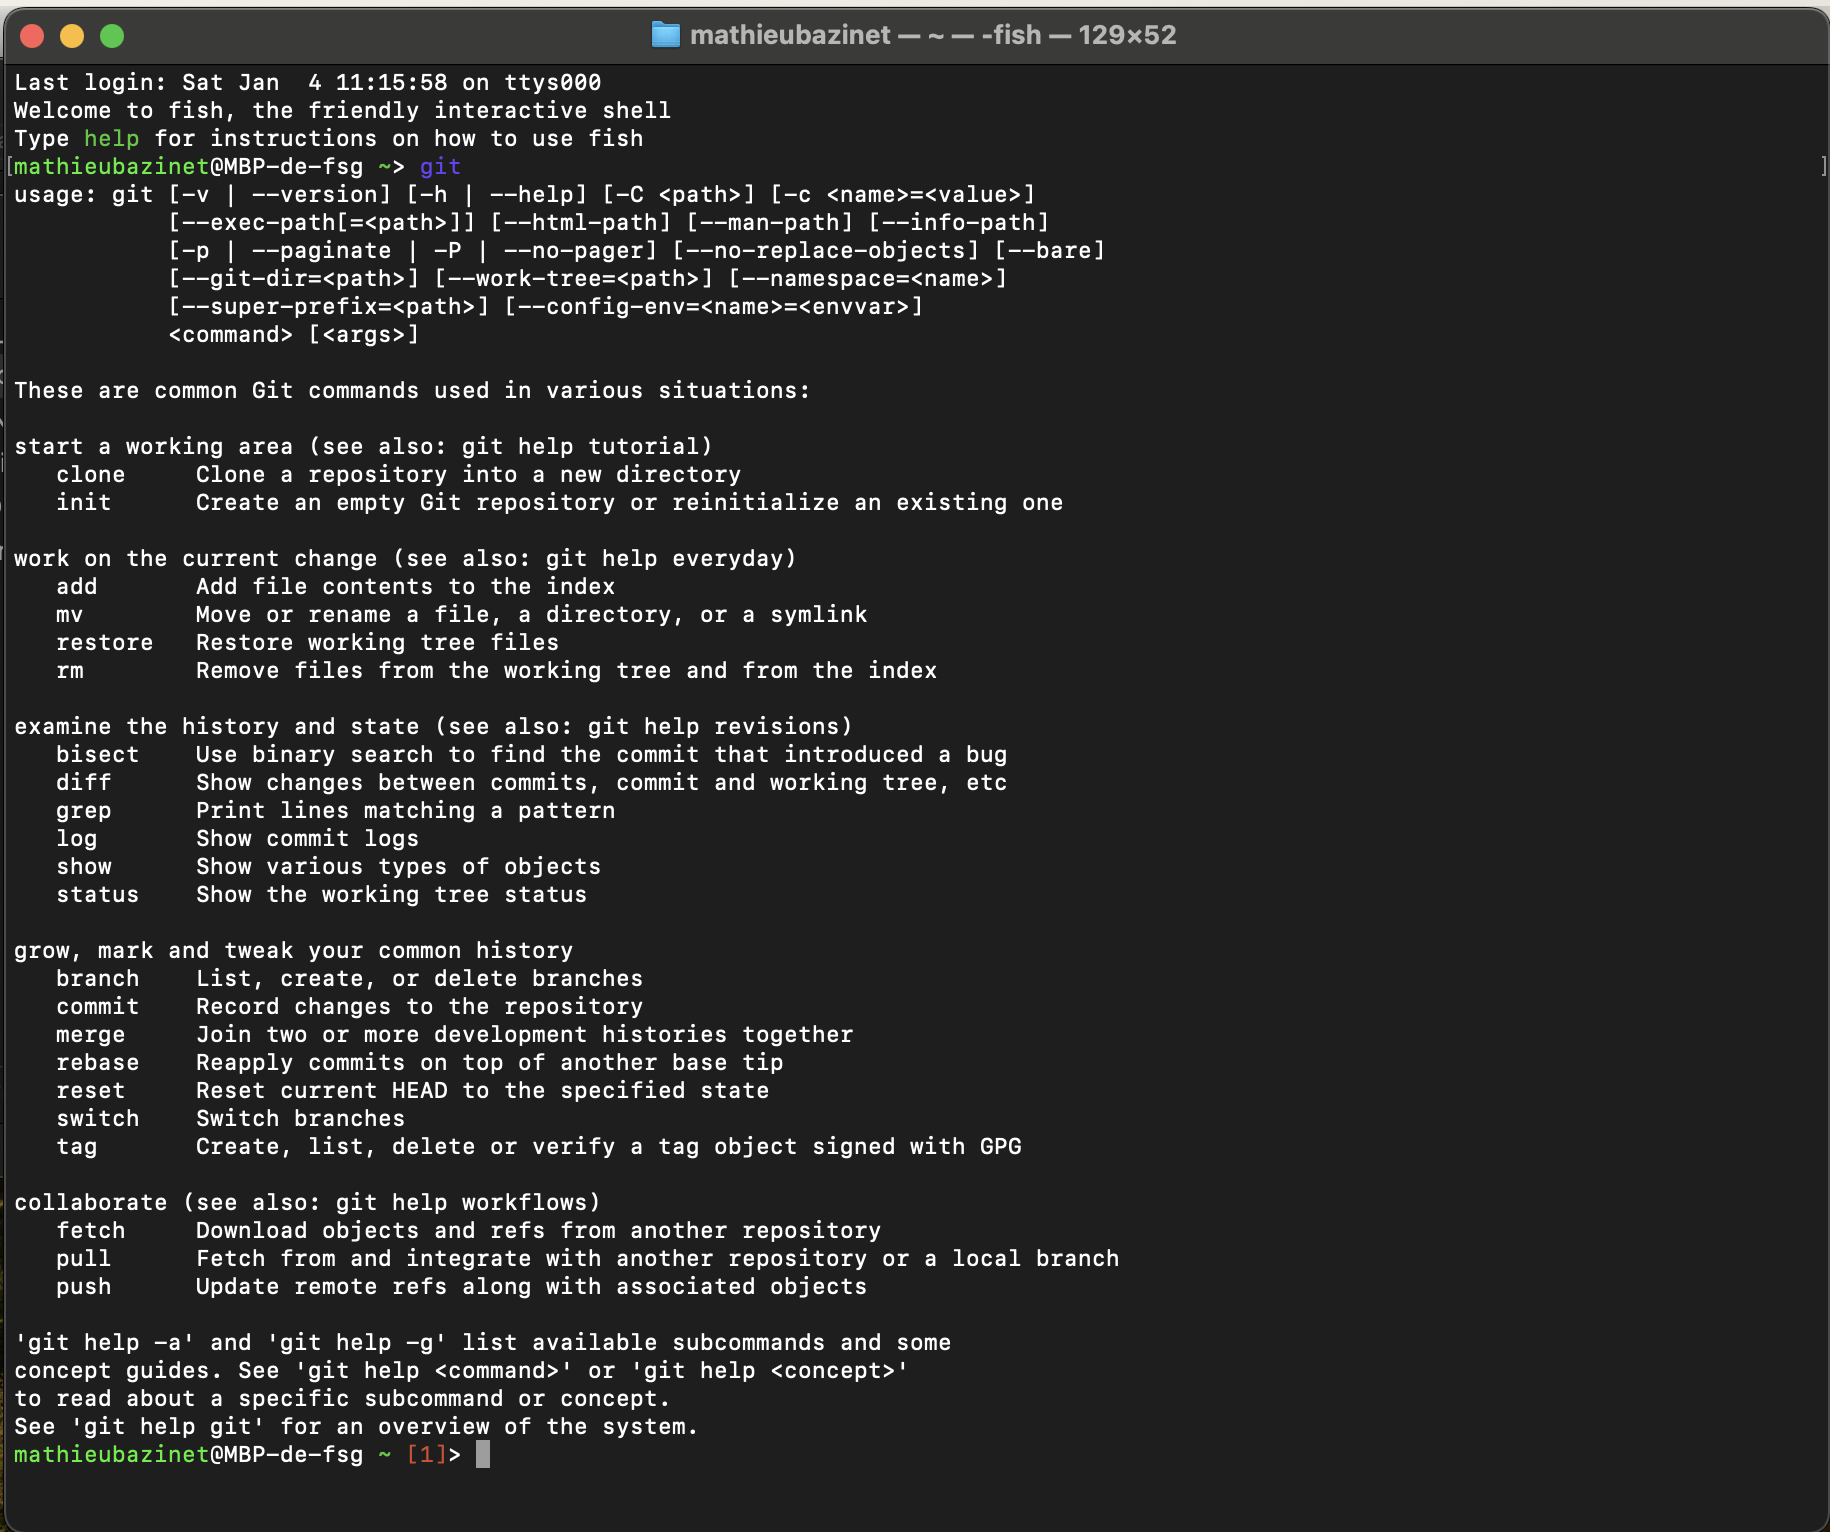
\includegraphics[width=0.8\textwidth]{images/check_if_git.png}
    \caption{Sortie attendue dans le terminal lorsque la commande ``git'' est tapée dans le terminal.} \label{fig:check_if_git}
\end{figure}
Download : 
	\url{https://git-scm.com/}
	xcode-select --install

Configuring git :
\begin{lstlisting}
	git config --global user.email "votre_courriel@ulaval.ca"
	git config --global user.name "votre_nom"
\end{lstlisting}
token d’identification (Mac) (\url{https://docs.github.com/fr/authentication/keeping-your-account-and-data-secure/managing-your-personal-access-tokens\#cr%C3%A9ation-dun-personal-access-token-classic}) 



\section{Première étape avec Git}

Cloner le repo de ce tutoriel
aller chercher le lien du repo

\begin{figure}[!h]
    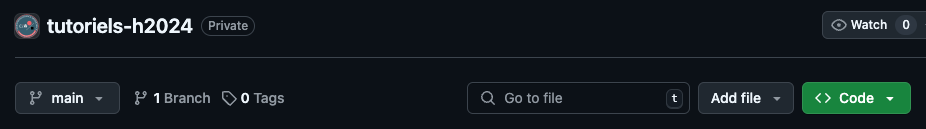
\includegraphics[width=\textwidth]{images/clone_button_github.png}
    \caption{À remplir} \label{fig:clone_button}
\end{figure}

cloner un repo
\begin{lstlisting}
    git clone https://github.com/cia-ulaval/tutoriels-h2024.git
\end{lstlisting}


\begin{definition}
    La commande \texttt{\emph{git clone <url-du-repo>}} permet de créer une copie locale du projet. 
\end{definition}

\end{document}